\documentclass[12pt]{article}

\usepackage{sbc-template}
\usepackage{cite}
\usepackage{graphicx,url}
\usepackage[utf8]{inputenc}
\usepackage[brazil]{babel} 
     
\sloppy

\title{Aplicação de \textit{Automatic Number Plate Recognition} (ANPR) no controle de acesso de veículos}

\author{Maurício de Abreu Cordeiro\inst{1}, Alexandro Santos Silva\inst{1} }

\address{Instituto Federal de Educação, Ciência e Tecnologia da Bahia\\ 
	Avenida Sérgio Vieira Melo, 3150. Bairro Zabelê - Vitória da Conquista - BA - Brasil\\
	CEP 45078-900
  \email{mauriciocordeiro@live.com, alexandrossilva@ifba.edu.br}
}

\begin{document} 

\maketitle

\begin{abstract}
  This paper describes the development of an access control system, based on ANPR (Automatic Number Plate Recognition) technologies, with a large potencial of application in physical spaces which demands some security level for access (such as condominium complex and parking lots). The system follows a design based on Microservices Architecture, alongside Docker containers and comunication through HTTP following REST principles.
\end{abstract}
     
\begin{resumo} 
 Este trabalho descreve o desenvolvimento de um sistema para controle de acesso de veículos baseado em ANPR (\textit{Automatic Number Plate Recognition}), com largo potencial de sua aplicação em locais ou espaços físicos que exigem algum nível de segurança, quando da entrada e saída de pessoas (a título de exemplo, citam-se aqui condomínios e estacionamentos privados). O sistema segue um desenho arquitetural baseado em microsserviços, com contêineres Docker e comunicação via HTTP seguindo os princípios REST.
\end{resumo}

\section{Introdução}

Atualmente, já se tornou comum encontrar ambientes com vídeo-monitoramento, sejam eles interno ou externos. Além disso, os avanços no poder computacional e em técnicas de processamento, detecção e classificação de imagens fez surgir inúmeras possibilidades de incutir semântica e expandir a aplicabilidade de visão computacional em situações do dia a dia.

Nesse cenário, uma das aplicações possíveis é o uso de câmeras para capturar imagens de placas de veículos que passam por guaritas ou portões e, a partir da identificação de sua placa, liberar ou não seu acesso. A tecnologia utilizada para tal é chamada de ANPR (\textit{Automatic Number Plate Recognition}).

Assim, a proposta desse trabalho consiste na implementação de um sistema de controle de acesso com interface \textit{web}, aplicação de ANPR e baseado na arquitetura de microsserviços para a manutenção de uma lista de veículos permitidos, bem como a sua verificação a partir de processamento de imagem.

\subsection{Trabalhos correlatos}

Em \citen{felix2017entry}, o ANPR é aplicado em um Circuito Fechado de TV para o monitoramento de entrada e saída de veículos em um ambiente. A solução apresentada utiliza processamento de imagem com MATLAB, OCR (Optical Character Recognition) e rede neural para classificação de imagens e caractéres.

\citen{matysiak2013analysis} propõem o uso de câmeras com tecnologias de ANPR para monitorar e punir eventuais infrações de trânsito em faixas exclusivas para tráfego de ônibus, na cidade de Varsóvia, na Polônia.

\citen{aalsalem2017campussense} apresentam um sistema para monitoramento de estacionamento, com mapeamento e busca de veículos a partir da aplicação de ANPR.

\section{Arquitetura} \label{sec:architecture}

A solução desenvolvida neste trabalho baseia-se na arquitetura de microsserviços, com módulos virtuais conteinerizados, que se comunicam via HTTP, além da aplicação de tecnologias baseadas em ANPR. Esta seção se dedica a detalhar esses conceitos.

\subsection{Arquitetura de Microsserviços}

Arquitetura de Microsserviços (\textit{Microservices Architecture} - MSA) é um modelo arquitetural onde processos de \textit{software} são realizados por componentes fracamente acoplados, que possuem funcionalidades específicas e bem definidas, e que se comunicam através de interfaces padronizadas \cite{viggiato2018}.

A MSA pode ser considerada como a segunda iteração da Arquitetura Orientada a Serviços (\textit{Service Oriented Architecture} - SOA), onde serviços complexos são decompostos em partes mais flexíveis, especializadas e de fácil manutenção, de modo que cada uma é responsável por uma única e pequena funcionalidade com o intuito de realizá-la bem \cite{homay2019}. 

\subsection{Virtualização baseada em contêiner}

A Virtualização baseada em contêiner \cite{eder2016} consiste na utilização de recursos de \textit{hardware} e do \textit{kernel} de um sistema hospedeiro a fim de criar ambientes isolados para a execução de determinados processos, o chamado \textbf{contêiner}, conforme esquematizado na Figura~\ref{fig:conteiner}.

\begin{figure}[ht]
	\centering
	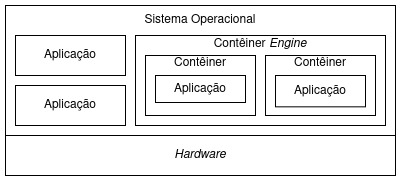
\includegraphics[width=1\textwidth]{conteiner.jpg}
	\caption{Virtualização baseada em contêiner}
	\label{fig:conteiner}
\end{figure} 

Nessa abordagem, o contêiner aloca apenas os recursos necessários para executar sua aplicação, de modo a trabalhar isolado de outros contêineres que possam estar em execução em um mesmo hospedeiro. Essa característica corrobora com sua utilidade quanto a aplicação em soluções baseadas em MSA, uma vez que os contêineres são capazes de se comunicar entre si.

\subsection{REST}

O REST (\textit{REpresentational State Transfer}) é uma implementação da SOA sobre o HTTP para transferência de representações de um determinado recurso entre cliente e servidor \cite{mumbaikar2013}.

De forma geral, o REST estabelece semântica para métodos e URI (\textit{Universal Resource Identifier}) no HTTP, padronizando a forma como recursos são solicitados e disponibilizados na web (Figura~\ref{fig:rest}). Nesse contexto, leia-se "recurso" como um item acessível via URI, e a "semântica do método" padroniza o modo de interação com o recurso, podendo se associar, por exemplo, \texttt{POST} à criação, \texttt{GET} à solicitação, \texttt{PUT} à edição e \texttt{DELETE} à remoção\cite{adamczyk2011}.

\begin{figure}[ht]
	\centering
	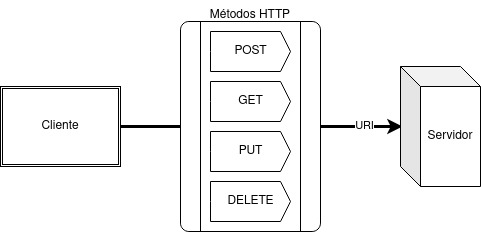
\includegraphics[width=.8\textwidth]{rest.jpg}
	\caption{Comunicação cliente-servidor com REST}
	\label{fig:rest}
\end{figure} 

\subsection{ANPR}

O ANPR (\textit{Automatic Number Plate Recognition}), que possui papel central na solução desenvolvida neste trabalho, é uma tecnologia que utiliza visão computacional e processamento de imagem para identificar e reconhecer caracteres em placas de veículos.

Existem diferentes técnicas e algoritmos que podem ser usados no ANPR, mas, de forma geral, todos eles seguem um processo com etapas bem definidas \cite{mufti2021}: (i) Extração da placa, (ii) Segmentação de caracteres e (iii) Reconhecimento de caracteres.

Em cada uma das etapas para a execução do ANPR, \cite{shashirangana2020} pode-se empregar diferentes técnicas (que vão desde algoritmos de processamento de imagens até aplicação de redes neurais para classificação de objetos), conforme o mostrado na Figura~\ref{fig:anpr-steps}:

\begin{figure}[ht]
	\centering
	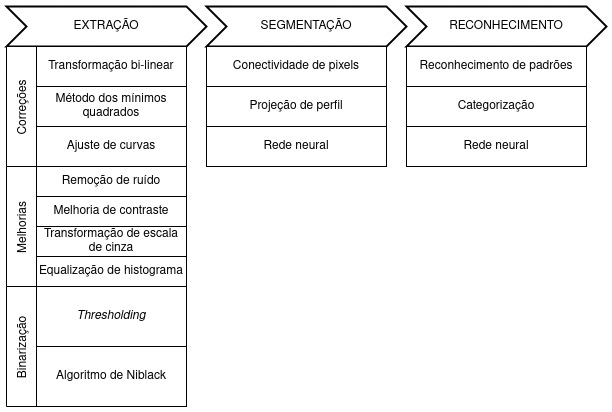
\includegraphics[width=1\textwidth]{anpr-steps.jpg}
	\caption{Etapas e técnicas aplicadas no ANPR}
	\label{fig:anpr-steps}
\end{figure} 

\section{Implementação}

O sistema para controle de acesso de veículos implementado neste trabalho foi organizado em módulos, ou contêineres, cada um com uma funcionalidade específica (seguindo os princípios da MSA), e se comunicando direta ou indiretamente entre si, como mostrado na Figura~\ref{fig:anpr-auth}. Esses módulos foram implementados com o uso de diversas linguagens, \textit{frameworks} e ferramentas, a saber: Docker, Java, Python, Angular e MongoDB.

\begin{figure}[ht]
	\centering
	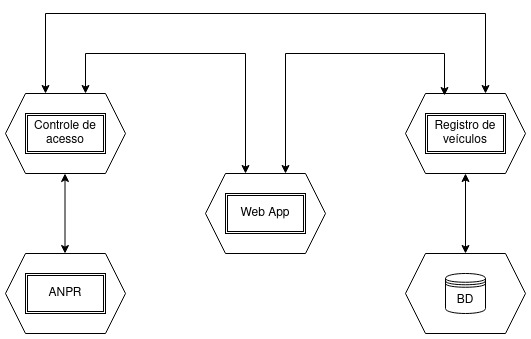
\includegraphics[width=.8\textwidth]{anpr-auth.jpg}
	\caption{Esquema da organização e relacionamento entre os contêineres do sistema}
	\label{fig:anpr-auth}
\end{figure}

A seguir, será apresentada com detalhes a forma com que cada um dos módulos foi desenvolvido e como eles se interagem.

\subsection{Composição de contêineres}

Todos os módulos do sistema são construídos com contêineres Docker, a partir de imagens padrão ou personalizadas, constituindo assim uma aplicação multi-conteiner.

Para definir e executar a aplicação com múltiplos contêineres, é utilizada a ferramenta Docker Compose\footnote{Página para a documentação oficial do Docker Compose: \url{https://docs.docker.com/compose/}}. Essa ferramenta tem o objetivo de otimizar o processo de construção e execução de múltiplos contêineres, tanto das etapas de desenvolvimento e testes quanto da implantação para produção.

O uso da ferramenta consiste em 3 passos:

\begin{enumerate}
	\item Definir, no arquivo \textit{Dockerfile}, os recursos necessários de cada um dos contêineres da aplicação, como a imagem docker, dependências, usuários e diretórios, portas de serviços e comandos para execução de aplicações, etc. De forma geral, o \textit{Dockerfile} é um \textit{script} que define \textbf{quais} e \textbf{como} instalar e utilizar as ferramentas e aplicações de um contêiner;
	\item Definir, em um arquivo \textit{.yml}, os serviços necessários e a relação entre os contêineres, como interfaces de rede, portas de serviços, volumes de disco e dependências entre contêineres;
	\item Executar o comando \texttt{docker-compose up} para inicializar todos os contêineres descritos no arquivo \textit{.yml}
\end{enumerate}

Vale ressaltar que, apesar do controle ser realizado em um unico arquivo, o Docker Compose, em um cenário de atualização, apenas reconstruirá o contêiner que possuir alguma modificação.

\subsection{ANPR}

O módulo ANPR é o responsável por realizar o processamento das imagens dos veículos e devolver o texto de sua placa. Para tal, foi utilizada a biblioteca de código-aberto OpenALPR\footnote{Endereço do repositório e documentação da biblioteca: \url{https://github.com/openalpr/openalpr}} e foi implementada uma API REST com o \textit{framework} Java Spring-Boot para processar as requisições de leitura de placas e devolver respostas, no formato JSON\footnote{JavaScript Object Notation.}, para o contêiner cliente.

A Figura~\ref{fig:anpr4j-data} ilustra o fluxo das requisições de leitura de placa para a API do contêiner de ANPR.

\begin{figure}[ht]
	\centering
	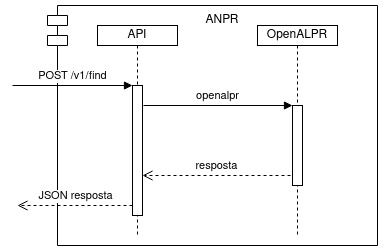
\includegraphics[width=.6\textwidth]{anpr4j-data.jpg}
	\caption{Fluxo de requisições no contêiner de ANPR}
	\label{fig:anpr4j-data}
\end{figure}

A biblioteca OpenALPR, ao receber uma imagem, realiza uma série de etapas para detectar o possível texto escrito na placa do veículo \cite{openalprdesign}:

\begin{enumerate}
	\item \textbf{Detecção:} busca de regiões com possíveis placas na imagem;
	\item \textbf{Binarização:} transformação em preto-e-branco as regiões de possíveis placas;
	\item \textbf{Análise de caractéres:} busca por possíveis caractéres na imagem;
	\item \textbf{Análise de bordas:} busca pelas bordas da placa na região;
	\item \textbf{Ajuste de distorção:} corrige a perspectiva da placa, para que seja "vista de frente";
	\item \textbf{Segmentação:} segmentação individual dos caractéres na placa;
	\item \textbf{OCR:} análise da imagem de cada caractére para encontrar a letra ou número correspondente;
	\item \textbf{Pós-processamento:} criação de um \textit{ranking} de placas detectadas, com base na confiança e espressões regulares (se solicitado).
\end{enumerate}

A resposta do OpenALPR é então capturada pela API e enviada ao contêiner solicitante.

\subsection{Banco de Dados (BD)}

Este é o módulo responsável pela persistência dos dados usados pelo sistema, construído com uma imagem do MongoDB\footnote{Página oficial do MongoDB: \url{https://www.mongodb.com/}. Página para a imagem Docker do MongoDB: \url{https://hub.docker.com/_/mongo}}. Ele se encontra em um contêiner próprio para fins de controle de eventuais atualizações e uso de volume de disco, uma vez que a lógica da persistência dos dados se encontra no módulo descrito na sub-seção seguinte.

\subsection{Registro de veículos}

Este é o módulo responsável pela lógica de persistência do sistema e acesso ao banco de dados.

Escrito em Python, este módulo implementas as operações CRUD\footnote{\textit{Create}, \textit{Read}, \textit{Update} e \textit{Delete}} para veículos e usuários do sistema — utilizando a biblioteca PyMongo\footnote{Documentação oficial do PyMongo: \url{https://docs.mongodb.com/drivers/pymongo/}} —, enquanto implementa uma API — com a biblioteca Flask\footnote{Documentação oficial do Flask: \url{https://flask.palletsprojects.com/en/2.0.x/}}—, para tratar as requisições de outros módulos.

\subsection{Controle de acesso}

O módulo de Controle de acesso — escrito em Java com Spring-Boot — é onde a principal lógica de negócio do sistema está implementada. Ele é responsável por receber, via requisição REST, uma imagem de uma aplicação cliente qualquer, repassar esta imagem para o módulo ANPR para obter a placa do veículo e então requisitar ao módulo de Registros as informações de cadastro referentes à placa encontrada. De posse dessas informações, ele responde a aplicação cliente informando se o veículo da imagem tem ou não a autorização de acesso.

O diagrama da Figura~\ref{fig:check4j} ilustra a troca de mensagens encabeçada pelo módulo de Controle de acesso.

\begin{figure}[ht]
	\centering
	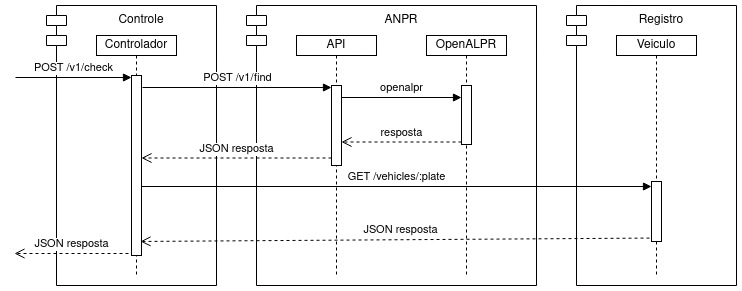
\includegraphics[width=1\textwidth]{check4j.jpg}
	\caption{Fluxo de requisições a partir do Controle de acesso}
	\label{fig:check4j}
\end{figure}

\subsection{\textit{Web App}}

O módulo \textit{Web App}, escrito em TypeScript com o \textit{framework} Angular 9, interpreta dois papéis no sistema implementado: (i) \textit{front-end} para a manutenção das informações de cadastro de veículos, acessando o módulo Registro de veículos; e (ii) \textit{front-end} para prova de conceito do sistema, realizando requisições para o módulo de Controle de acesso.

Além se poder ser executado em um contêiner Docker, este módulo pode ser compilado como um aplicativo móvel multiplataforma\footnote{Android ou iOS} através do \textit{framework} Apache Cordova\footnote{Documentação oficial do Apache Cordova: \url{https://cordova.apache.org/docs/en/latest/}}.

\section{Resultados}

O principal objetivo deste trabalho foi implementar um sistema que utilize tecnologias de ANPR baseada em uma arquitetura MSA e que utilize ferramentas amplamente adotadas pela comunidade de desenvolvimento de \textit{software}. Os resultados obtidos são apresentados como se segue.

A construção da infraestrutura interna e a definição das portas de comunicação entre contêineres é realizada, através do \textit{Docker Compose} e de seu arquivo de configuração, conforme apresentado anteriormente. Uma vez executado, os 5 contêineres que representam o sistema devem estar acessíveis da seguinte forma:

\begin{itemize}
\item \textit{Web App}: \texttt{anpr-ng:4000} ou \texttt{localhost:4000};
\item Controle de acesso: \texttt{check4j:8081} ou \texttt{localhost:8081};
\item Registro de veículos: \texttt{vehiclespy:5001} ou \texttt{localhost:5001};
\item ANPR: \texttt{alpr4j:8080} ou \texttt{localhost:8080};
\item Banco de dados: \texttt{db:27017} ou \texttt{localhost:27017}.
\end{itemize}

Com o objetivo de demonstrar o conceito do sistema, o módulo \textit{Web Apps} possui três formulários principais: (i) Listagem de veículos, (ii) Cadastro de veículos — apresentados na Figura~\ref{fig:vehicles-forms} — e (iii) Verificação de autorização — na Figura~\ref{fig:check-form}.

\begin{figure}[ht]
	\centering
	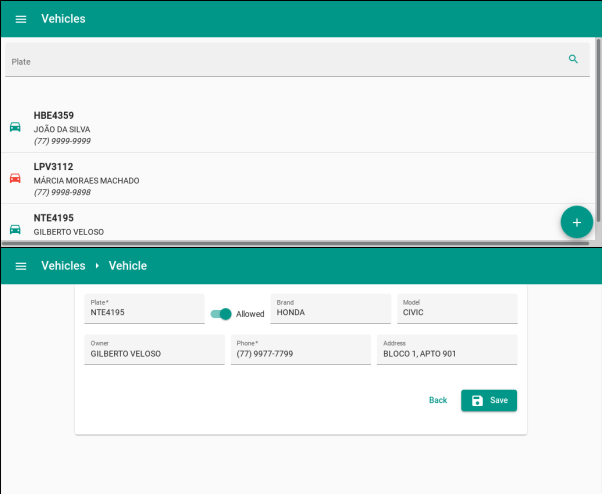
\includegraphics[width=1\textwidth]{vehicles-forms.png}
	\caption{Formulários de exibição e cadastro de veículos.}
	\label{fig:vehicles-forms}
\end{figure}

\begin{figure}[ht]
	\centering
	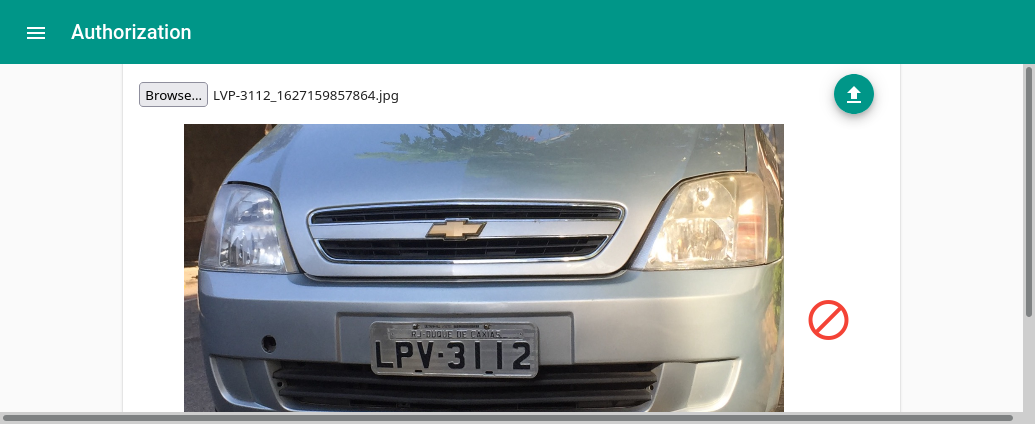
\includegraphics[width=1\textwidth]{check-form.png}
	\caption{Formulário de verificação de autorização.}
	\label{fig:check-form}
\end{figure}

\section{Trabalhos Futuros}

O sistema implementado neste trabalho, apesar de ter cumprido os objetivos propostos, possui alguns pontos de melhoria que podem sem tratados em trabalhos futuros, como:

\begin{itemize}
	\item \textbf{Integração com periféricos de entrada e saída}, a exemplo de câmeras de monitoramento para captura de imagem e vídeo de veículos e com catracas eletrônicas para liberação de veículos;
	\item \textbf{Otimização de gestão e escalabilidade}, pela utilização de ferramentas como Kubernetes\footnote{Documentação oficial do Kubernetes \url{https://kubernetes.io/docs/home/}}, para melhor gerenciamento e escalabilidade dos contêineres;
	 \item \textbf{Melhoria de performance no módulo de ANPR:} Estudos podem ser realizados neste ponto, com a substituição do contêiner \texttt{alpr4j} por outro com uma metodologia diferente de ANPR, com uso de redes neurais que passam por treinamento de acordo com o ambiente onde o sistema será implantado, a fim de melhorar a precisão dos resultados fornecidos pelo módulo;
	 \item \textbf{IaC e PaaS:} Implementar uma solução de IaC (\textit{Infrastructure as Code}), como o Terraform\footnote{Documentação oficial do Terraform: \url{https://www.terraform.io/docs/index.html}}, para gerenciar a construção e implantação do sistema em nuvem (PaaS - Platform as a Service).
\end{itemize}

\bibliographystyle{sbc}
\bibliography{sbc-template}

\end{document}
